\documentclass[12pt]{article}
\usepackage{hyperref}

\usepackage{graphicx}

\usepackage{mathtools}
\DeclarePairedDelimiter\ceil{\lceil}{\rceil}
\DeclarePairedDelimiter\floor{\lfloor}{\rfloor}

\usepackage{xcolor}

\usepackage{amsmath}
\usepackage{amsfonts}
\usepackage{amssymb}

\newcommand{\Mod}[1]{\ (\mathrm{mod}\ #1)}


\usepackage{listings}
\lstset{language=C++,
  basicstyle=\fontsize{8}{13}\ttfamily,
  keywordstyle=\color{blue}\ttfamily,
  stringstyle=\color{red}\ttfamily,
  commentstyle=\color{green}\ttfamily,
  morecomment=[l][\color{magenta}]{\#}
}

\usepackage{breqn}
\usepackage[]{algorithm2e}
\usepackage{physics}

\newcommand\fnurl[2]{%
  \href{#2}{#1}\footnote{\url{#2}}%
}

\newcommand{\Four}{\mathcal{F}}
\renewcommand{\(}{\left(}
\renewcommand{\)}{\right)}
%% \renewcommand{\{}{\left{}
%% \renewcommand{\}}{\right}}


\title{API design for rocFFT/hipFFT}
\author{The rocFFT Team}



\def\no#1{\nobreak{#1}} % stop equation breaking in dmath

\begin{document}
\maketitle

\section{Introduction}

FIXME \texttt{rocFFT}.

\section{DAG}


\begin{center}
  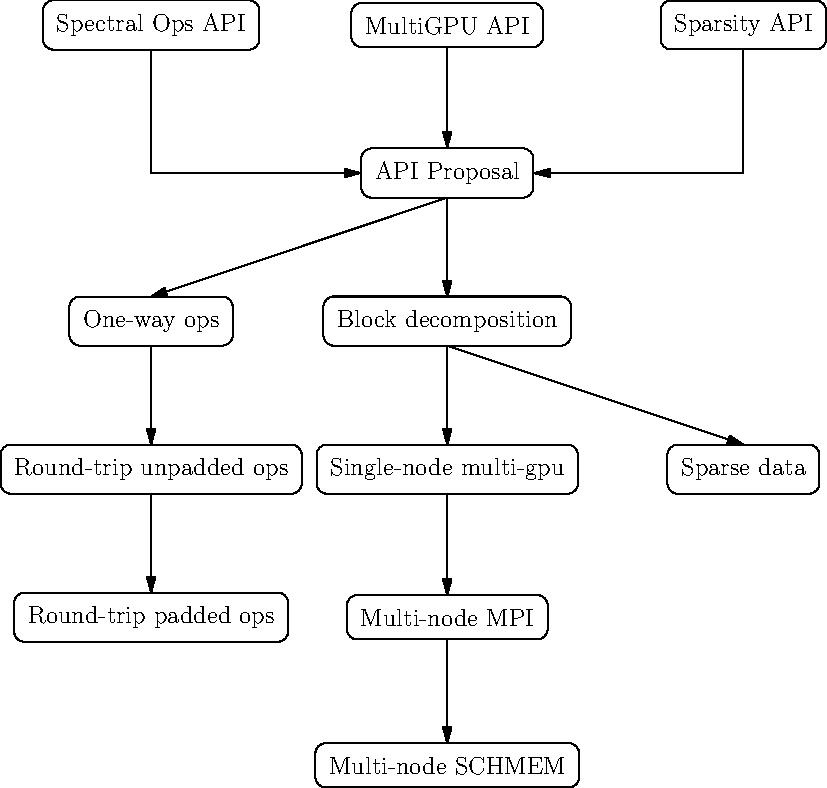
\includegraphics[width=0.9\textwidth]{implementdag.pdf}
\end{center}

\newpage
\subsection{Fields}
\label{ssfields}

\noindent
Dependencies:
\begin{itemize}
\item None
\end{itemize}

\noindent
Status:
\begin{itemize}
\item Implimented in ROCm 6.0
\end{itemize}

\noindent
rocFFT API additions:
\begin{lstlisting}
typedef struct rocfft_field_t* rocfft_field;
rocfft_status rocfft_field_create(rocfft_field* field);
rocfft_status rocfft_field_destroy(rocfft_field field);
rocfft_status rocfft_plan_description_add_infield(rocfft_plan_description description,
                                                 rocfft_field            field);
rocfft_status rocfft_plan_description_add_infield(rocfft_plan_description description,
                                                 rocfft_field            field);

rocfft_status
    rocfft_plan_description_add_outfield(rocfft_plan_description description, rocfft_field field);
\end{lstlisting}

hipFFT API additions:
\begin{lstlisting}
FIXME
\end{lstlisting}

\newpage
\subsection{Bricks}
\label{ssbricks}

Dependencies:
\begin{itemize}
\item Field (see \ref{ssfields})
\end{itemize}

Status:
\begin{itemize}
\item Experimental implementation in ROCm 6.0
\end{itemize}

Optional:
\begin{itemize}
\item FIXME
\end{itemize}

\noindent
rocFFT API additions:
\begin{lstlisting}
typedef struct rocfft_brick_t* rocfft_brick;
rocfft_status rocfft_brick_create(rocfft_brick* brick,
                                  const size_t* field_lower,
                                  const size_t* field_upper,
                                  const size_t* brick_stride,
                                  size_t        dim,
                                  int           deviceID);
rocfft_status rocfft_brick_destroy(rocfft_brick brick);
rocfft_status rocfft_field_add_brick(rocfft_field field, rocfft_brick brick);
\end{lstlisting}

hipFFT API additions:
\begin{lstlisting}
FIXME
\end{lstlisting}

\newpage
\subsection{Single-Process Multi-GPU}

Dependencies:
\begin{itemize}
\item Bricks (see \ref{ssbricks})
\end{itemize}

\noindent
Status:
\begin{itemize}
\item Experimental implementation in ROCm 6.0
\end{itemize}

\noindent
Optional:
\begin{itemize}
\item Specify a specific list of GPUs to use:
\begin{lstlisting}
rocfft_status rocfft_plan_description_set_devices( rocfft_plan_description description,
                                                   void *devices,
                                                   size_t number_of_devices);
\end{lstlisting}
\end{itemize}


\noindent
rocFFT API additions: implied by brick-device association.

\noindent
hipFFT API additions:
\begin{lstlisting}
FIXME
\end{lstlisting}

\newpage
\subsubsection{Multi-Process Multi-GPU}

Dependencies:
\begin{itemize}
\item Bricks (see \ref{ssbricks})
\end{itemize}

\noindent
Status:
\begin{itemize}
\item Scoped for development starting in 6.1
\end{itemize}

\noindent
Optional:
\begin{itemize}
\item FIXME
\end{itemize}


\noindent
rocFFT API additions: implied by brick-device association.
\begin{lstlisting}
typedef enum rocfft_comm_type_t {
} rocfft_comm_type;
rocfft_status rocfft_plan_description_set_comm(
    rocfft_plan_description description,
    const enum_type_for_mpi_or_schmem comm_type,
    void* comm_handle);
\end{lstlisting}

\noindent
hipFFT API additions:
\begin{lstlisting}
FIXME
\end{lstlisting}

\newpage
\subsubsection{Multi-Process Multi-GPU with MPI}

Dependencies:
\begin{itemize}
\item Bricks (see \ref{ssbricks})
\end{itemize}

\noindent
Status:
\begin{itemize}
\item Scoped for development starting in 6.1
\end{itemize}

\noindent
Optional:
\begin{itemize}
\item FIXME
\end{itemize}


\noindent
rocFFT API additions:
\begin{lstlisting}
typedef enum rocfft_comm_type_t {
  rocfft_comm_mpi = 0,
} rocfft_comm_type;
\end{lstlisting}

\noindent
hipFFT API additions:
\begin{lstlisting}
FIXME
\end{lstlisting}

\newpage
\subsubsection{Multi-Process Multi-GPU with rocSHMEM}

Dependencies:
\begin{itemize}
\item Bricks (see \ref{ssbricks})
\end{itemize}

\noindent
Status:
\begin{itemize}
\item Unscoped.   Working on performance model for BU justification.
\end{itemize}

\noindent
Optional:
\begin{itemize}
\item FIXME
\end{itemize}


\noindent
rocFFT API additions:
\begin{lstlisting}
typedef enum rocfft_comm_type_t {
    rocfft_comm_shmem = 1,
} rocfft_comm_type;
\end{lstlisting}

\noindent
hipFFT API additions:
\begin{lstlisting}
FIXME
\end{lstlisting}

\newpage
\subsection{Sparse Data}

Dependencies:
\begin{itemize}
\item Bricks (see \ref{ssbricks})
\end{itemize}

\noindent
Status:
\begin{itemize}
\item Unscoped.
\end{itemize}

\noindent
Optional:
\begin{itemize}
\item FIXME
\end{itemize}


\noindent
rocFFT API additions:
\begin{lstlisting}
  FIXME
\end{lstlisting}

\noindent
hipFFT API additions:
\begin{lstlisting}
  FIXME
\end{lstlisting}

\newpage
\subsection{Spectral Ops}

\newpage
\subsubsection{One-Way Scalar Spectral Ops}

Dependencies:
\begin{itemize}
\item Bricks (see \ref{ssbricks})
\end{itemize}

\noindent
Status:
\begin{itemize}
\item Unscoped.
\end{itemize}

\noindent
Optional:
\begin{itemize}
\item FIXME
\end{itemize}


\noindent
rocFFT API additions:
\begin{lstlisting}
  FIXME
\end{lstlisting}

\noindent
hipFFT API additions:
\begin{lstlisting}
  FIXME
\end{lstlisting}
\newpage
\subsubsection{One-Way Multi-valued Spectral Ops}

Dependencies:
\begin{itemize}
\item Bricks (see \ref{ssbricks})
\end{itemize}

\noindent
Status:
\begin{itemize}
\item Unscoped.
\end{itemize}

\noindent
Optional:
\begin{itemize}
\item FIXME
\end{itemize}


\noindent
rocFFT API additions:
\begin{lstlisting}
  FIXME
\end{lstlisting}

\noindent
hipFFT API additions:
\begin{lstlisting}
  FIXME
\end{lstlisting}
\newpage
\subsubsection{Round Trip Multi Spectral Ops Without Padding}

Dependencies:
\begin{itemize}
\item Bricks (see \ref{ssbricks})
\end{itemize}

\noindent
Status:
\begin{itemize}
\item Unscoped.
\end{itemize}

\noindent
Optional:
\begin{itemize}
\item FIXME
\end{itemize}


\noindent
rocFFT API additions:
\begin{lstlisting}
  FIXME
\end{lstlisting}

\noindent
hipFFT API additions:
\begin{lstlisting}
  FIXME
\end{lstlisting}
\newpage
\subsection{Round Trip Multi Spectral Ops With Padding}

Dependencies:
\begin{itemize}
\item Bricks (see \ref{ssbricks})
\end{itemize}

\noindent
Status:
\begin{itemize}
\item Unscoped.
\end{itemize}

\noindent
Optional:
\begin{itemize}
\item FIXME
\end{itemize}


\noindent
rocFFT API additions:
\begin{lstlisting}
  FIXME
\end{lstlisting}

\noindent
hipFFT API additions:
\begin{lstlisting}
  FIXME
\end{lstlisting}

\end{document}
